\documentclass[tikz,border=10pt]{standalone}

\usepackage{verbatim}

\begin{document}
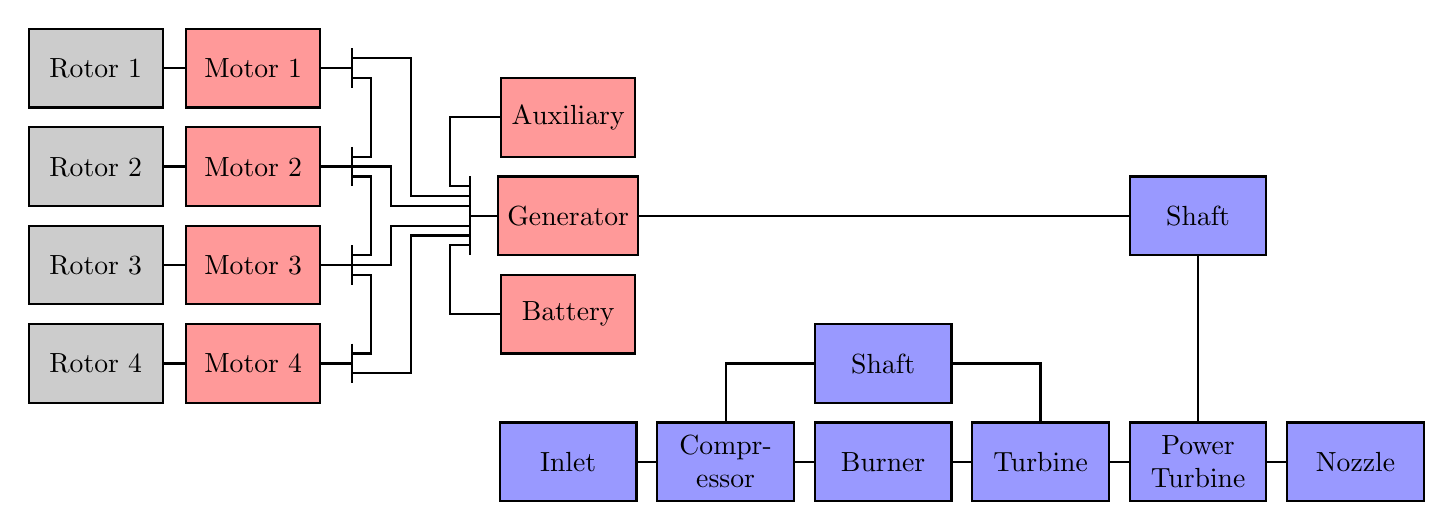
\begin{tikzpicture}[node distance = 1.2cm, thick, nodes = {align = center}, >=latex]

  \tikzstyle{rotor}=[draw, rectangle, minimum height=1cm, minimum width=1.7cm, fill=gray!40,]
  \tikzstyle{elec}=[draw, rectangle, minimum height=1cm, minimum width=1.7cm, fill=red!40,]
  \tikzstyle{cycle}=[draw, rectangle, minimum height=1cm, minimum width=1.7cm, text width=1.5cm, fill=blue!40,]

  % Prop/rotor
  \node[rotor] (r1) at (0,5.00) {Rotor 1};
  \node[rotor] (r2) at (0,3.75) {Rotor 2};
  \node[rotor] (r3) at (0,2.50) {Rotor 3};
  \node[rotor] (r4) at (0,1.25) {Rotor 4};

  % Electrical
  \node[elec] (m1) at (2.0,5.00) {Motor 1};
  \node[elec] (m2) at (2.0,3.75) {Motor 2};
  \node[elec] (m3) at (2.0,2.50) {Motor 3};
  \node[elec] (m4) at (2.0,1.25) {Motor 4};
  \node[elec] (aux) at (6,4.375) {Auxiliary};
  \node[elec] (gen) at (6,3.125) {Generator};
  \node[elec] (batt) at (6,1.875) {Battery};

  % Cycle
  \node[cycle] (inlet) at (6,0) {Inlet};
  \node[cycle] (comp) at (8,0) {Compr-essor};
  \node[cycle] (burn) at (10,0) {Burner};
  \node[cycle] (turb) at (12,0) {Turbine};
  \node[cycle] (pt) at (14,0) {Power Turbine};
  \node[cycle] (nozz) at (16,0) {Nozzle};
  \node[cycle] (hp_shaft) at (10,1.25) {Shaft};
  \node[cycle] (lp_shaft) at (14,3.125) {Shaft};

  % Buses
  \draw (3.25,5.25) -- (3.25,4.75);
  \draw (3.25,4.0) -- (3.25,3.5);
  \draw (3.25,2.75) -- (3.25,2.25);
  \draw (3.25,1.5) -- (3.25,1.0);
  \draw (4.75,2.625) -- (4.75,3.625);

  % Lines between rotors and motors
  \draw (r1) -- (m1);
  \draw (r2) -- (m2);
  \draw (r3) -- (m3);
  \draw (r4) -- (m4);

  % Lines between motors and buses
  \draw (m1) -- (3.25,5.0);
  \draw (m2) -- (3.25,3.75);
  \draw (m3) -- (3.25,2.5);
  \draw (m4) -- (3.25,1.25);

  % Lines between generator and bus
  \draw (gen) -- (4.75,3.125);

  % Lines for cross wing cables
  \draw (3.25,1.25+0.125) -- (3.5,1.25+0.125) -- (3.5,2.5-0.125) -- (3.25,2.5-0.125);
  \draw (3.25,2.5+0.125) -- (3.5,2.5+0.125) -- (3.5,3.75-0.125) -- (3.25,3.75-0.125);
  \draw (3.25,3.75+0.125) -- (3.5,3.75+0.125) -- (3.5,5.0-0.125) -- (3.25,5.0-0.125);

  % Lines for major cables
  \draw (3.25,1.25-0.125) -- (4.0,1.25-0.125) -- (4.0,3.125-0.25) -- (4.75,3.125-0.25);
  \draw (3.25,5.0+0.125) -- (4.0,5.0+0.125) -- (4.0,3.125+0.25) -- (4.75,3.125+0.25);
  \draw (3.25,2.5) -- (3.75,2.5) -- (3.75,3.125-0.125) -- (4.75,3.125-0.125);
  \draw (3.25,3.75) -- (3.75,3.75) -- (3.75,3.125+0.125) -- (4.75,3.125+0.125);
  \draw (batt) -- (4.5,1.875) -- (4.5,3.125-0.375) -- (4.75,3.125-0.375);
  \draw (aux) -- (4.5,4.375) -- (4.5,3.125+0.375) -- (4.75,3.125+0.375);

  % Lines between cycle elements
  \draw (inlet) -- (comp);
  \draw (comp) -- (burn);
  \draw (burn) -- (turb);
  \draw (turb) -- (pt);
  \draw (pt) -- (nozz);
  \draw (comp) -- (8,1.25) -- (hp_shaft);
  \draw (turb) -- (12,1.25) -- (hp_shaft);
  \draw (gen) -- (lp_shaft);
  \draw (pt) -- (lp_shaft);

\end{tikzpicture}
\end{document}